
\chapter{Materiais e Métodos}
\label{metodologia}
Este capítulo descreve o modo como a pesquisa, desenvolvimento e a documentação
do framework sugerido na \autoref{objetivos} será conduzida.

\section{Tecnologias utilizadas}
A escolha das tecnologias segue de acordo com a arquitetura do sistema.

\subsection{Javascript}
Para desenvolvimento do \emph{Framework} será utilizada a linguagem \emph{Javascript},
uma linguagem altamente difundida para desenvolvimento de páginas web.

Nos últimos anos a linguagem passou a ser usada também para desenvolvimento de
aplicações para servidor.


\subsection{Node.js}
Será utilizado o \emph{Node.js} como plataforma de execução do framework, ele
conta com recursos nativos do Sistema Operacional o que o torna extremamente
viável para o framework.


\subsection{Desenvolvimento}
Ao final do desenvolvimento, deveremos ter uma Aplicação, para realizar o
processamento das tarefas distribuídas, e um \emph{Framework} capaz de distribuir
tarefas em outras máquinas.


\subsubsection{Conexão}
O \emph{Framework} em sua inicialização receberá as informações, como
endere\c{c}o e detalhes de autenticação dos servidores que contém a aplicação que
processará as tarefas. A conexão, segundo o modelo de \citeonline{tanenbaum},
deve ser realizada utilizando o protocolo \emph{RTP}, um protocolo de
comunicação em tempo real baseado no protocolo \emph{UDP}, mas a implementação
será realizada utilizando o protocolo \emph{UDP}.


\subsubsection{Distribui\c{c}\~{a}o de tarefas}
O \emph{Framework} utilizará classes para:
\begin{itemize}
  \item Criação das tarefas;
  \item Configuração das tarefas;
  \item Distribuição das tarefas;
\end{itemize}

O fluxo da distribuição de tarefas seguirá o modelo da figura \ref{fig:dist-tarefas}.

Toda distribuição feita pela aplicação utilizando o framework deverá ser feita
por mensagens conforme o modelo a seguir:


\begin{lstlisting}[language=json, firstnumber=1]
{
  "id": Number,
  "start": Number,
  "size": Number,
  "dependencies": [String],
  "script": String
}
\end{lstlisting}

Onde \emph{``id''} será o código identificador utilizado internamente pela
aplicação, \emph{``start''} e \emph{``size''} delimitadores para o paralelismo
nos múltiplos computadores, \emph{``dependencies''} os \emph{pacotes}
necessários pelo processo e \emph{``script''} sendo o algoritmo que será
executado para cada conjunto de dados.

\begin{figure}[htb]
	\caption{\label{fig:dist-tarefas}Fluxo de tarefas distribuídas}
	\begin{center}
		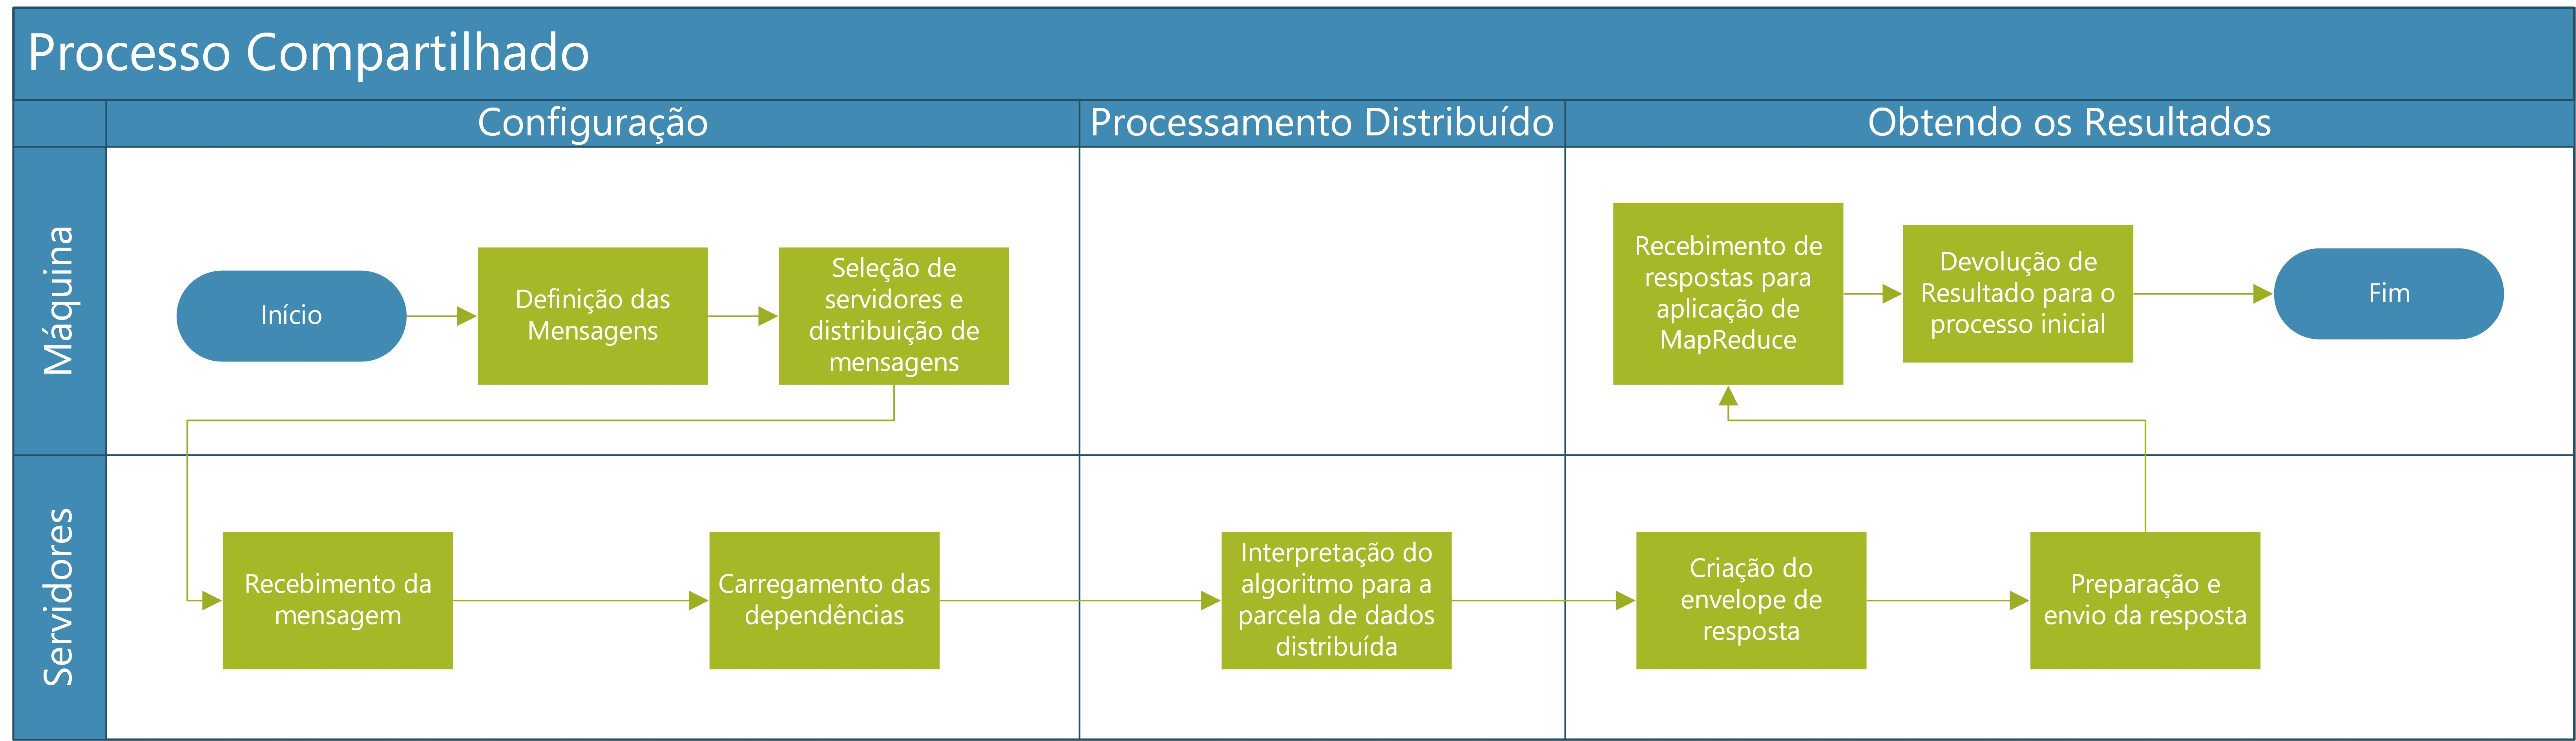
\includegraphics[width=1\textwidth]{img/processamento-distribuido.jpg}
	\end{center}
	\legend{Fonte: Elaborada pelo autor.}
\end{figure}

O processo de criação de uma chamada de procedimento remoto foi desenvolvido
tendo como base o modelo composto pelas etapas descritas por \citeonline{tanenbaum} na
figura \ref{fig:criacao-chamada}.

\begin{figure}[htb]
	\caption{\label{fig:criacao-chamada}Etapas na criação de uma chamada de procedimento remoto}
	\begin{center}
		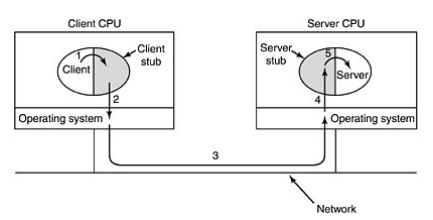
\includegraphics[width=1\textwidth]{img/criacao-chamada.jpg}
	\end{center}
	\legend{Fonte: Tanenbaum (2013).}
\end{figure}

A injeção de dependências será realizada internamente pelo servidor no processo
de carregamento de dependências seguindo o modelo da
figura \ref{fig:injecao-dependencias}.

\begin{figure}[htb]
	\caption{\label{fig:injecao-dependencias}Modelo de injeção de dependências}
	\begin{center}
		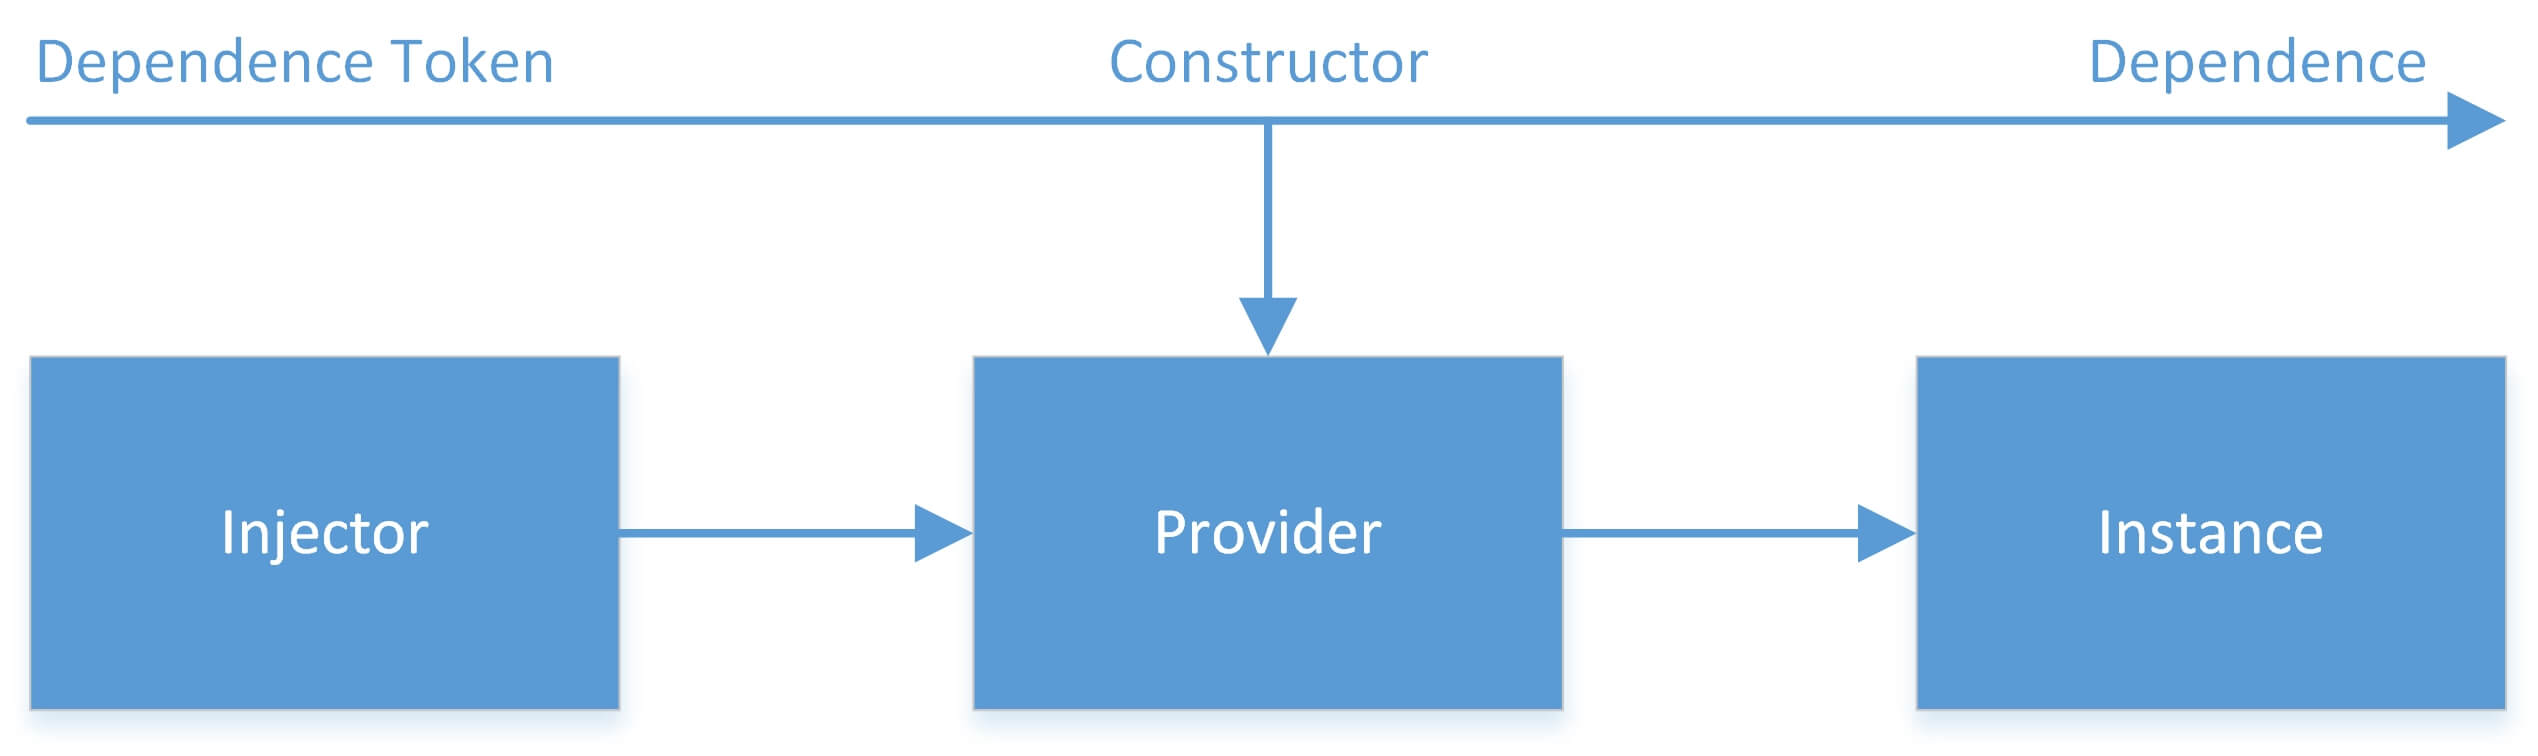
\includegraphics[width=1\textwidth]{img/injecao-dependencias.jpg}
	\end{center}
	\legend{Fonte: Elaborada pelo autor.}
\end{figure}

\pagebreak
\subsubsection{Aplicação para execução das tarefas}
A aplicação para distribuição também será feita utilizando \emph{Javascript} e
\emph{Node.js}. Ela interpretará a tarefas recebida e responderá para o
\emph{Framework} se ela foi executada corretamente ou não. Em caso de
\emph{MapReduce} também responderá com os dados processados.

\section{Padrões de Projeto}
O sistema utiliza os seguintes padrões de projeto baseados nos padrões de projeto da gangue
dos quatro definido no livro ``Design Patterns''.

\begin{itemize}
  \item \textbf{Command:} Modelo utilizado para padronização da execução interna
  de tarefas bem definidas, como inicialização e interrupção de processos;
  \item \textbf{Observer:} Modelo utilizado para aguardar mudanças na rede, como
  pedidos de execução de algoritmos, implementado no sistema em conjunto com o
  modelo de Command;
  \item \textbf{Factory:} Modelo utilizado para definir um padrão ao gerar
  objetos com bases em comum. Como no caso a criação e injeção de dependências.
\end{itemize}


Devido a utilização de uma linguagem interpretada, com poucos recursos de uma
linguagem orientada a objetos, se torna inviável a utilização de herança e fluxo
de informação à risca dos mesmos.

\section{Documentação}
Além da aplicação será necessário uma documentação bem descrita do código-fonte
e da arquitetura do sistema, abaixo serão descritas as ferramentas responsáveis
por esse requisito

\subsection{JSDoc}
\emph{JSDoc} é uma ferramenta utilizada para documentação de código-fonte em
\emph{Javascript}. A partir de comentários dentro do código-fonte é compilado um
conjunto de documentos responsáveis por descrever os \emph{módulos},
\emph{classes} e \emph{métodos} do código-fonte. Abaixo nas figuras
\ref{fig:jsdoc-js} e \ref{fig:jsdoc-html} exemplificam a entrada e saída de uma
documentação JSDoc.

\begin{figure}[htb]
	\caption{\label{fig:jsdoc-js}Exemplo de comentários no código-fonte para documentação}
	\begin{center}
		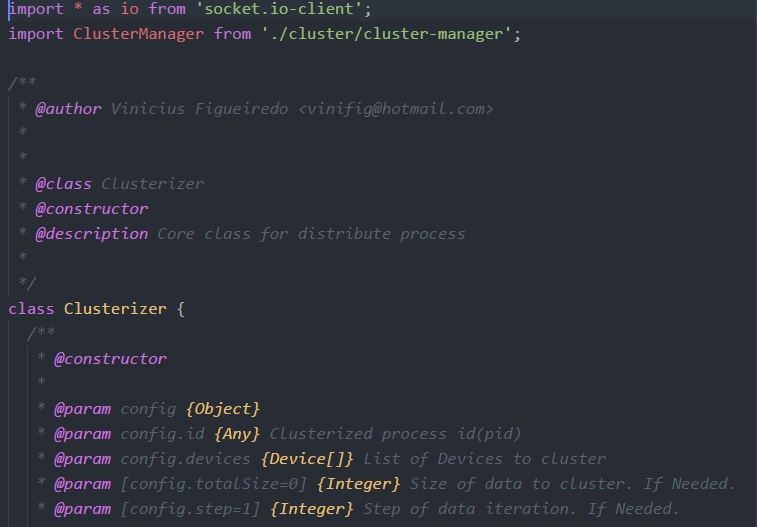
\includegraphics[width=1\textwidth]{img/jsdoc-js.jpg}
	\end{center}
	\legend{Fonte: Elaborada pelo autor.}
\end{figure}

\begin{figure}[htb]
	\caption{\label{fig:jsdoc-html}Exemplo de documento gerado pelo JSDoc}
	\begin{center}
		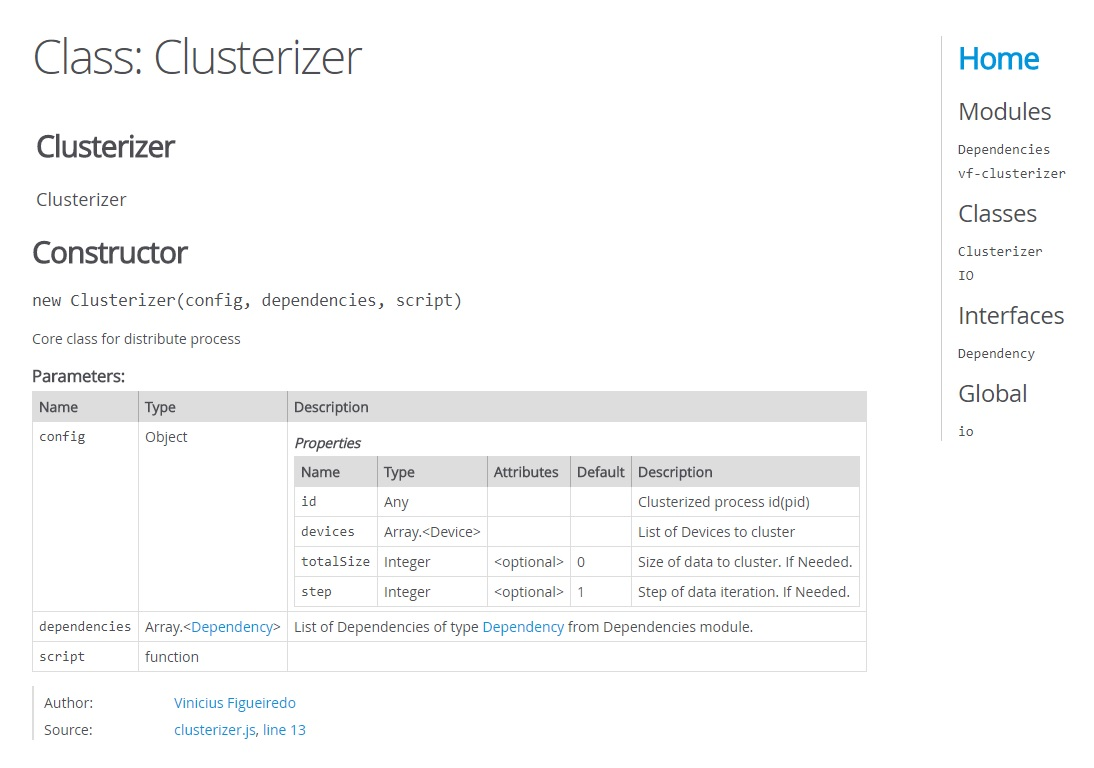
\includegraphics[width=1\textwidth]{img/jsdoc-html.jpg}
	\end{center}
	\legend{Fonte: Elaborada pelo autor.}
\end{figure}

\section{Protótipo}
Os requisitos funcionais definidos para o protótipo do sistema são:

\begin{itemize}
  \item Capacidade de comunicação entre as máquinas.
  \item Execução de comandos simples em outra máquina ou instância de software;
  \item Tratamento de erros de conexão.
  \item Documentação completa ou parcial do código-fonte existente.
\end{itemize}

Foram desenvolvidos um framework, responsável por auxiliar a comunicação da
aplicação \emph{client-side} com a aplicação \emph{server-side}. Abaixo na
figura \ref{fig:prototipo-resultado}, mostra um exemplo da execução da aplicação
definida na figura \ref{fig:prototipo-trecho-fonte} onde retorna
o horário em que foi executado cada iteração da tarefa distribuída.

\begin{figure}[htb]
	\caption{\label{fig:prototipo-trecho-fonte}Exemplo de código para
  distribuição de tarefas}
	\begin{center}
		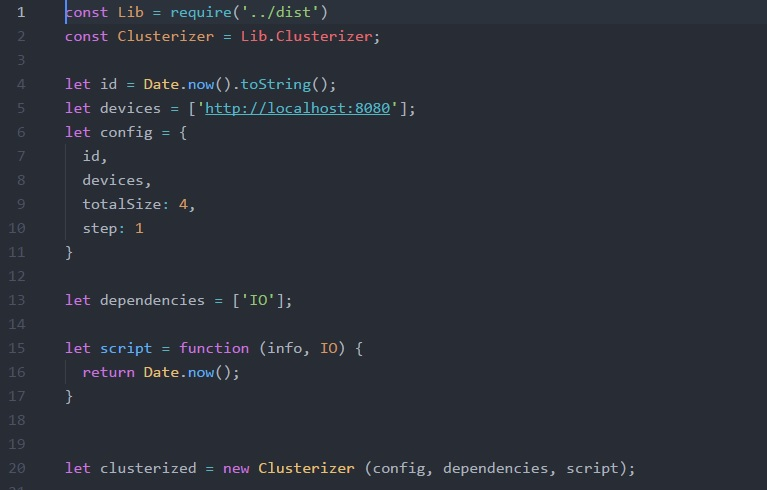
\includegraphics[width=1\textwidth]{img/prototipo-trecho-fonte.jpg}
	\end{center}
	\legend{Fonte: Elaborada pelo autor.}
\end{figure}

\begin{figure}[htb]
	\caption{\label{fig:prototipo-resultado}Exemplo de retorno de tarefa
  distribuída}
	\begin{center}
		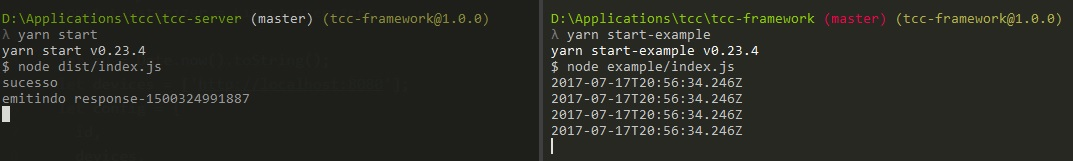
\includegraphics[width=1\textwidth]{img/prototipo-resultado.jpg}
	\end{center}
	\legend{Fonte: Elaborada pelo autor.}
\end{figure}
